This section presents the definitions of the physics objects used in the analysis: electrons, muons, jets and \ensuremath{E_{\mathrm{T}}^{\mathrm{miss}}}.  
The flavour tagging selection ($b$-tagging), together with the overlap removal procedure of the considered objects are also presented. 
All these objects are selected/reconstructed as implemented  in \texttt{AnalysisTop 21.2.169}.

%=========================================================
\subsection{Electrons}
\label{subsec:obj-electrons}
%=========================================================

Electron candidates are reconstructed as described in
Chapter~\ref{ch:reco}. In this analysis, prompt isolated electrons
are selected using the likelihood-based \texttt{TightLH}
identification working point, together with kinematic, impact-parameter,
and isolation requirements optimised for heavy-object decays.
Electrons are required to satisfy transverse-momentum and pseudorapidity
criteria within the well-instrumented calorimeter acceptance,
excluding the barrel–endcap transition region.
To ensure compatibility with the hard-scatter interaction,
constraints on the transverse and longitudinal impact parameters
with respect to the primary vertex are imposed.
Non-prompt backgrounds are further suppressed by applying the
\texttt{FCTight} isolation working point.
In the same-sign dilepton channels, an additional multivariate
charge-identification requirement (ECIDS) is applied to reduce
backgrounds from charge misidentification.
Residual efficiency differences between data and simulation
are corrected by applying the standard reconstruction,
identification, isolation, trigger, and charge-identification
scale factors to simulated events.

Two electron definitions are used in the analysis:
a \textit{tight} selection used in signal and control regions,
and a \textit{loose} selection used for overlap removal and
background studies. The detailed requirements are summarised
in Tables~\ref{tab:object:electron} and~\ref{tab:object:loose_electron}.

\begin{table}[ht]
  \caption{Tight electron selection used in the analysis.}
  \label{tab:object:electron}
  \centering
  \begin{tabular}{ll}
    \toprule
    Requirement & Definition \\
    \midrule
    Kinematic acceptance &
    $p_{\mathrm{T}} > 28~\mathrm{GeV}$ \\
    &
    $(|\eta| < 1.37)\; \text{or}\; (1.52 < |\eta| < 2.47)$ \\
    \midrule
    Identification & \texttt{TightLH} \\
    \midrule
    Isolation &
    \texttt{FCTight} \\
    &
    $\texttt{topoetcone20}/p_T < 0.06$ \\
    &
    $\texttt{ptvarcone20\_TightTTVA\_pt1000}/p_T < 0.06$ \\
    \midrule
    Impact parameter &
    $|d_0/\sigma(d_0)| < 5$ \\
    &
    $|\Delta z_0 \sin\theta| < 0.5~\mathrm{mm}$ \\
    \midrule
    Object quality &
    Standard ATLAS electron quality requirements \\
    \midrule
    Charge identification &
    ECIDS (same-sign channels only) \\
    \bottomrule
  \end{tabular}
\end{table}

\begin{table}[ht]
  \caption{Loose electron selection used for overlap removal and background studies.}
  \label{tab:object:loose_electron}
  \centering
  \begin{tabular}{ll}
    \toprule
    Requirement & Definition \\
    \midrule
    Kinematic acceptance &
    $p_{\mathrm{T}} > 10~\mathrm{GeV}$ \\
    &
    $(|\eta| < 1.37)\; \text{or}\; (1.52 < |\eta| < 2.47)$ \\
    \midrule
    Identification & \texttt{MediumLH} \\
    \midrule
    Isolation & Not required \\
    \midrule
    Impact parameter &
    $|d_0/\sigma(d_0)| < 5$ \\
    &
    $|\Delta z_0 \sin\theta| < 0.5~\mathrm{mm}$ \\
    \midrule
    Object quality &
    Standard ATLAS electron quality requirements \\
    \midrule
    Charge identification &
    ECIDS (same-sign channels only) \\
    \bottomrule
  \end{tabular}
\end{table}

%%%%%%%%%%%%%%%%%%%%%%%%%%%%%%%%%%%%%%%%%%%%%
%NOTES:
% Selection: /cvmfs/atlas.cern.ch/repo/sw/software/21.2/AnalysisBase/21.2.120/InstallArea/x86_64-centos7-gcc8-opt/src/PhysicsAnalysis/TopPhys/xAOD/TopObjectSelectionTools/Root/ElectronLikelihoodMC15.cxx
% Calibration: /cvmfs/atlas.cern.ch/repo/sw/software/21.2/AnalysisBase/21.2.120/InstallArea/x86_64-centos7-gcc8-opt/src/PhysicsAnalysis/TopPhys/xAOD/TopCPTools/Root/TopEgammaCPTools.cxx
% Isolation: /cvmfs/atlas.cern.ch/repo/sw/software/21.2/AnalysisBase/21.2.120/InstallArea/x86_64-centos7-gcc8-opt/src/PhysicsAnalysis/AnalysisCommon/IsolationSelection/Root/IsolationSelectionTool.cx
%%%%%%%%%%%%%%%%%%%%%%%%%%%%%%%%%%%%%%%%%%%%%

%=========================================================
\subsection{Muons}
\label{subsec:obj-muons}
%=========================================================

Muon reconstruction in ATLAS is described in
Chapter~\ref{ch:reco}. In this analysis, prompt isolated muons
are selected using the \texttt{Medium} identification working
point, which provides a balance between efficiency and purity
over the relevant transverse-momentum range.

Selected muons are required to satisfy transverse-momentum and
pseudorapidity requirements within the fiducial inner-detector
acceptance. To ensure compatibility with the hard-scatter
interaction, constraints on the transverse and longitudinal
impact parameters with respect to the primary vertex are applied.
Non-prompt muons originating from heavy-flavour decays or
hadron misidentification are further suppressed using a
track-based isolation requirement.

Residual differences in trigger, reconstruction, identification,
isolation, and track-to-vertex-association efficiencies between
data and simulation are corrected by applying the standard
data-to-simulation scale factors to simulated events.

As for electrons, two muon definitions are used in the analysis:
a \textit{tight} selection used in signal and control regions,
and a \textit{loose} selection used for overlap removal and
dedicated background studies. The detailed requirements are
summarised in Tables~\ref{tab:object:muon} and
\ref{tab:object:loose_muon}.

\begin{table}[ht]
  \caption{Tight muon selection used in the analysis.}
  \label{tab:object:muon}
  \centering
  \begin{tabular}{ll}
    \toprule
    Requirement & Definition \\
    \midrule
    Kinematic acceptance &
    $p_{\mathrm{T}} > 28~\mathrm{GeV}$ \\
    &
    $|\eta| < 2.5$ \\
    \midrule
    Identification & \texttt{Medium} \\
    \midrule
    Isolation &
    \texttt{FCTightTrackOnly} \\
    &
    $\texttt{ptvarcone30\_TightTTVA\_pt1000}/p_T < 0.06$ \\
    \midrule
    Impact parameter &
    $|d_0/\sigma(d_0)| < 3$ \\
    &
    $|\Delta z_0 \sin\theta| < 0.5~\mathrm{mm}$ \\
    \bottomrule
  \end{tabular}
\end{table}

\begin{table}[ht]
  \caption{Loose muon selection used for overlap removal and background studies.}
  \label{tab:object:loose_muon}
  \centering
  \begin{tabular}{ll}
    \toprule
    Requirement & Definition \\
    \midrule
    Kinematic acceptance &
    $p_{\mathrm{T}} > 10~\mathrm{GeV}$ \\
    &
    $|\eta| < 2.5$ \\
    \midrule
    Identification & \texttt{Medium} \\
    \midrule
    Isolation & Not required \\
    \midrule
    Impact parameter &
    $|d_0/\sigma(d_0)| < 3$ \\
    &
    $|\Delta z_0 \sin\theta| < 0.5~\mathrm{mm}$ \\
    \bottomrule
  \end{tabular}
\end{table}

%%%%%%%%%%%%%%%%%%%%%%%%%%%%%%%%%%%%%%%%
%NOTES:
% For muon selection: /cvmfs/atlas.cern.ch/repo/sw/software/21.2/AnalysisBase/21.2.120/InstallArea/x86_64-centos7-gcc8-opt/src/PhysicsAnalysis/TopPhys/xAOD/TopObjectSelectionTools/Root/MuonMC15.cxx

% Isolation definition: /cvmfs/atlas.cern.ch/repo/sw/software/21.2/AnalysisBase/21.2.120/InstallArea/x86_64-centos7-gcc8-opt/src/PhysicsAnalysis/AnalysisCommon/IsolationSelection/Root/IsolationSelectionTool.cx

% For sagitta bias:  /cvmfs/atlas.cern.ch/repo/sw/software/21.2/AnalysisBase/21.2.120/InstallArea/x86_64-centos7-gcc8-opt/src/PhysicsAnalysis/MuonID/MuonIDAnalysis/MuonMomentumCorrections/Root/MuonCalibrationPeriodTool.cxx
%%%%%%%%%%%%%%%%%%%%%%%%%%%%%%%%%%%%%%%%

%The selection criteria are implemented in the \texttt{MuonSelectorTools-XX-XX-XX}\\
%with \texttt{MuonMomentumCorrections-XX-XX-XX}, 
%isolation in \texttt{IsolationSelection-XX-XX-XX} and \dzero and \(z_{0}\) cuts in \texttt{xAODTracking-XX-XX-XX}.
%The muon recommendations can be found in 
%\href{https://twiki.cern.ch/twiki/bin/view/AtlasProtected/MCPAnalysisGuidelinesMC16}{MCPAnalysisGuidelinesMC16}.

%=========================================================
\subsection{Jets}
\label{subsec:obj-jets}
%=========================================================

Jets are reconstructed using the anti-$k_t$ algorithm with a
radius parameter $R=0.4$ and particle-flow inputs, as described
in Chapter~\ref{ch:reco}. Selected jets are required to satisfy
transverse-momentum and pseudorapidity requirements within the
central detector acceptance.

To suppress jets originating from pile-up interactions, a jet–vertex
association requirement is applied to low-$p_T$ central jets.
Standard ATLAS jet-quality criteria are imposed to remove events
containing jets affected by detector noise or non-collision
backgrounds. Energy calibration and resolution corrections are
applied according to the standard ATLAS Run~2 recommendations.

In the 1L channel, sensitivity to boosted hadronic top-quark
decays from heavy resonances is enhanced by constructing
re-clustered large-$R$ jets (RC-jets).
These are formed by reclustering selected small-$R$ jets using the
anti-$k_t$ algorithm with $R=1.0$.
To suppress soft radiation and residual pile-up contributions,
a trimming procedure is applied.
RC-jets satisfying dedicated kinematic requirements are used as
hadronic top-quark candidates.
The detailed jet selection criteria are summarised in
Table~\ref{tab:object:jet}.

\begin{table}[ht]
  \caption{Small-$R$ jet selection used in the analysis.}
  \label{tab:object:jet}
  \centering
  \begin{tabular}{ll}
    \toprule
    Requirement & Definition \\
    \midrule
    Algorithm & Anti-$k_t$, $R=0.4$ \\
    Input & Particle-flow \\
    \midrule
    Kinematic acceptance &
    $p_{\mathrm{T}} > 25~\mathrm{GeV}$ \\
    &
    $|\eta| < 2.5$ \\
    \midrule
    Pile-up suppression &
    JVT Tight for $p_{\mathrm{T}} < 60~\mathrm{GeV}$, \\
    &
    $|\eta| < 2.4$ \\
    \midrule
    Jet quality & Standard ATLAS \texttt{LooseBad} cleaning \\
    \bottomrule
  \end{tabular}
\end{table}

\begin{table}[ht]
  \caption{Reclustered large-$R$ jet (RC-jet) selection in the 1L channel.}
  \label{tab:object:rcjet}
  \centering
  \begin{tabular}{ll}
    \toprule
    Requirement & Definition \\
    \midrule
    Reclustering algorithm & Anti-$k_t$, $R=1.0$ \\
    Inputs & Selected small-$R$ jets \\
    \midrule
    Grooming & Trimming ($p_T^{\mathrm{subjet}}/p_T^{\mathrm{RC}} > 0.05$) \\
    \midrule
    Kinematic acceptance &
    $p_{\mathrm{T}} > 200~\mathrm{GeV}$ \\
    &
    $|\eta| < 2.0$ \\
    \bottomrule
  \end{tabular}
\end{table}

% NOTES:
% Selection: /cvmfs/atlas.cern.ch/repo/sw/software/21.2/AnalysisBase/21.2.120/InstallArea/x86_64-centos7-gcc8-opt/src/PhysicsAnalysis/TopPhys/xAOD/TopObjectSelectionTools/Root/JetMC15.cxx 
% Calibration tag: /cvmfs/atlas.cern.ch/repo/sw/software/21.2/AnalysisBase/21.2.120/InstallArea/x86_64-centos7-gcc8-opt/src/Reconstruction/Jet/JetCalibTools/Root/JetCalibrationTool.cx
% Calibration configuration: /cvmfs/atlas.cern.ch/repo/sw/software/21.2/AnalysisBase/21.2.120/InstallArea/x86_64-centos7-gcc8-opt/src/PhysicsAnalysis/TopPhys/xAOD/TopCPTools/Root/TopJetMETCPTools.cxx

%=========================================================
\subsection{$b$-tagging}
\label{subsec:obj-btag}
%=========================================================

Jets containing $b$-hadrons are identified using the DL1r
flavour-tagging algorithm described in
Chapter~\ref{ch:reco}. The algorithm exploits lifetime-sensitive
information from tracks and reconstructed secondary vertices
associated with the jet.

In this analysis, a working point corresponding to a nominal
70\% $b$-jet efficiency in simulated $t\bar{t}$ events is used.
This choice provides a balance between signal efficiency and
background rejection in final states with multiple heavy-flavour
jets.

Residual differences between data and simulation in the tagging
efficiency and mis-tag rates for $b$-, $c$-, and light-flavour
jets are corrected by applying standard data-to-simulation
scale factors to simulated events.
The detailed $b$-tagging definition is summarised in
Table~\ref{tab:object:btag}.

\begin{table}[ht]
  \caption{$b$-tagging definition used in the analysis.}
  \label{tab:object:btag}
  \centering
  \begin{tabular}{ll}
    \toprule
    Requirement & Definition \\
    \midrule
    Jet collection & Small-$R$ particle-flow jets \\
    Kinematic acceptance &
    $p_{\mathrm{T}} > 25~\mathrm{GeV}$ \\
    &
    $|\eta| < 2.5$ \\
    \midrule
    Algorithm & DL1r \\
    Working point & 70\% $b$-jet efficiency \\
    \bottomrule
  \end{tabular}
\end{table}

%=========================================================
\subsection{Missing transverse momentum}
\label{subsec:obj-met}
%=========================================================

Missing transverse momentum ($\vec{E}^{\mathrm{miss}}_T$)
is reconstructed using the standard object-based ATLAS
definition described in Chapter~\ref{ch:reco}.
The hard term is formed from calibrated electrons,
muons, and jets passing the analysis selections,
while the soft term is constructed using
primary-vertex-associated tracks.

No additional selection requirement on the magnitude of
$E^{\mathrm{miss}}_T$ is imposed at the object-definition
level. The reconstructed $E^{\mathrm{miss}}_T$ is used
in the event reconstruction and kinematic observables.

%=========================================================
\subsection{Overlap removal}
\label{subsec:overlap-removal}
%=========================================================

To ensure a unique assignment of detector signals to reconstructed
physics objects and to avoid double counting of energy deposits
or tracks, an overlap-removal procedure is applied.
Electrons, muons, and jets passing the loose preselection
are processed sequentially according to angular distance
and shared-track criteria.

The procedure resolves ambiguities between leptons and jets
originating from the same physical object, such as
non-prompt leptons inside jets or jets reconstructed from
lepton energy deposits.
The distance metric used to define spatial overlap is
$\Delta R = \sqrt{(\Delta y)^2 + (\Delta\phi)^2}$,
where $y$ denotes rapidity.

The detailed overlap-removal sequence is summarised in
Table~\ref{tab:overlap_removal}.

\begin{table}[ht]
\caption{Overlap-removal procedure applied to electrons, muons, and jets.
In each step, objects satisfying the listed criteria are removed.}
\label{tab:overlap_removal}
\centering
\begin{tabular}{lll}
\toprule
Object removed & Against & Criterion \\
\midrule
Electron & Electron & Shared track, lower-$p_T$ electron removed \\

Muon     & Electron & Calo-muon with shared ID track \\

Electron & Muon     & Shared ID track \\

Jet      & Electron & $\Delta R < 0.2$ \\

Electron & Jet      & $\Delta R < 0.4$ \\

Jet      & Muon     & $\texttt{NumTrack} < 3$ and \\
         &          & (ghost-associated or $\Delta R < 0.2$) \\

Muon     & Jet      & $\Delta R < \min\!\left(0.4,\; 0.04 + \frac{10~\mathrm{GeV}}{p_T(\mu)}\right)$ \\

\bottomrule
\end{tabular}
\end{table}

%=========================================================
\subsection{Event Selection and Region Definition}
\label{sec:event_selection}
%=========================================================

After object reconstruction and overlap removal,
events are categorised according to the lepton multiplicity
and the jet and $b$-jet multiplicities.
The event selection is designed to exploit the high object
multiplicity characteristic of four-tops final states
while maintaining sensitivity across a wide range of signal
kinematics.

\subsubsection{Lepton channels}

Two complementary channels are defined:

\begin{itemize}
\item \textbf{1L channel:} events containing exactly one isolated
electron or muon, targeting semileptonic decays of the top quarks.

\item \textbf{2LOS channel:} events containing exactly two isolated
leptons with opposite electric charge, targeting dileptonic top-quark
decays.
\end{itemize}

The two channels are analysed separately due to their different
background compositions and kinematic properties.

%---------------------------------------------------------
\subsubsection{Baseline jet and $b$-jet requirements}
%---------------------------------------------------------

To enhance sensitivity to multi-top final states,
events in the 1L (2LOS) channel are required to contain
at least seven (five) small-$R$ jets,
of which at least two must be $b$-tagged using
the 70\% efficiency working point of the DL1r algorithm.

These requirements suppress backgrounds from processes
with lower jet multiplicity and exploit the large
heavy-flavour content expected in signal events.

%---------------------------------------------------------
\subsubsection{Region categorisation}
%---------------------------------------------------------

Events satisfying the baseline requirements are further
categorised according to the jet multiplicity and the number
of $b$-tagged jets.

To refine the heavy-flavour composition of the selected
samples, the $b$-jet multiplicity is defined simultaneously
using multiple $b$-tagging operating points (60\%, 70\%, and 85\%).
For each event, the numbers of tagged jets
$N_b^{60\%}$, $N_b^{70\%}$, and $N_b^{85\%}$
are computed.

Event categories are defined using a logical \textbf{AND}
combination of these multiplicities.
This approach allows the selection of event samples
with different heavy-flavour purities.
Tighter operating points preferentially select jets
with higher probability of originating from $b$-hadrons,
while looser operating points retain higher efficiency.

For example, the 3bH category requires
\[
N_b^{60\%} = 3, \quad
N_b^{70\%} = 3, \quad
N_b^{85\%} > 3 ,
\]
which selects events where the three jets tagged at the
70\% working point are also tagged by the tighter 60\%
working point, while additional jets satisfy the looser
85\% criterion.

The analysis regions are designed to fulfil different roles in the
statistical interpretation of the data. In particular, they are used
to constrain the dominant backgrounds, validate the modelling of the
simulation, and maximise the sensitivity to potential signal
contributions.

The dominant Standard Model background arises from $t\bar{t}$ production
in association with additional jets. As described in
Section~\ref{sec:nn_rew}, a dedicated reweighting procedure is applied
to improve the modelling of the $t\bar{t}$+jets background.
The reweighting is derived using regions with either low jet
multiplicity and large $b$-jet multiplicity, or large jet multiplicity
and low $b$-jet multiplicity, where the potential signal contamination
is verified to be negligible.

Events in regions with at least three $b$-tagged jets are used in the
statistical analysis. Two multivariate discriminants are developed,
as described in Section~\ref{sec:mva}, and are used throughout the
analysis. The MVA output distributions, together with the
$H_\mathrm{T}$ distribution in selected regions, are included in a
simultaneous profile likelihood fit.

A total of 21 regions are used in the fit, consisting of 12 regions in
the 1L channel and 9 regions in the 2LOS channel. These regions are
defined by requiring at least eight (six) jets in the 1L (2LOS)
channel and satisfying the 3bL, 3bH, or $\ge4$b requirements.

Among these regions, those with at least ten (eight) jets, or with nine
(seven) jets and satisfying the $\ge4$b requirement in the
1L (2LOS) channel, are defined as signal regions (SRs). The remaining
fitted regions are defined as control regions (CRs), which primarily
constrain the normalisation and modelling of the background
contributions.

In addition, six validation regions (VRs) are defined by requiring at
least eight (six) jets in the 1L (2LOS) channel and satisfying the
3bV requirement. These regions are not included in the likelihood fit
and are used only to validate the modelling of the background
prediction.

The complete set of jet multiplicity and $b$-tagging multiplicity definitions used
to construct the event categories is summarised in
Table~\ref{tab:regions}.

%---------------------------------------------------------
\begin{table}[htbp]
  \centering
  \caption{
    Definition of the jet multiplicity and $b$-jet multiplicity requirements
    used to define the event categories.
    Events must satisfy all listed conditions simultaneously.
    $N_b^{60\%}$, $N_b^{70\%}$ and $N_b^{85\%}$
    denote the number of jets tagged at the corresponding
    operating points.
  }
  \begin{tabular}{m{6em}m{5em}m{5em}m{5em}}
    \hline
    \\[-1em]
    Name & $N_b^{60\%}$ & $N_b^{70\%}$ & $N_b^{85\%}$ \\
    \\[-1em]
    \hline
    2b             & -       & = 2     & - \\
    3bL            & $\le 2$ & = 3     & - \\
    3bH            & = 3     & = 3     & $> 3$ \\
    3bV            & = 3     & = 3     & = 3 \\
    $\ge$4b (2LOS) & -       & $\ge 4$ & - \\
    4b (1L)        & -       & = 4     & - \\
    $\ge$5b (1L)   & -       & $\ge 5$ & - \\
    \hline
  \end{tabular}
  \label{tab:regions}
\end{table}
%---------------------------------------------------------

The region definitions in the 1L and 2LOS channels
are illustrated schematically in
Fig.~\ref{fig:regions}.
The axes represent the jet multiplicity and
the $b$-tagging requirements described above.

%---------------------------------------------------------
\begin{figure}[htbp]
  \centering
  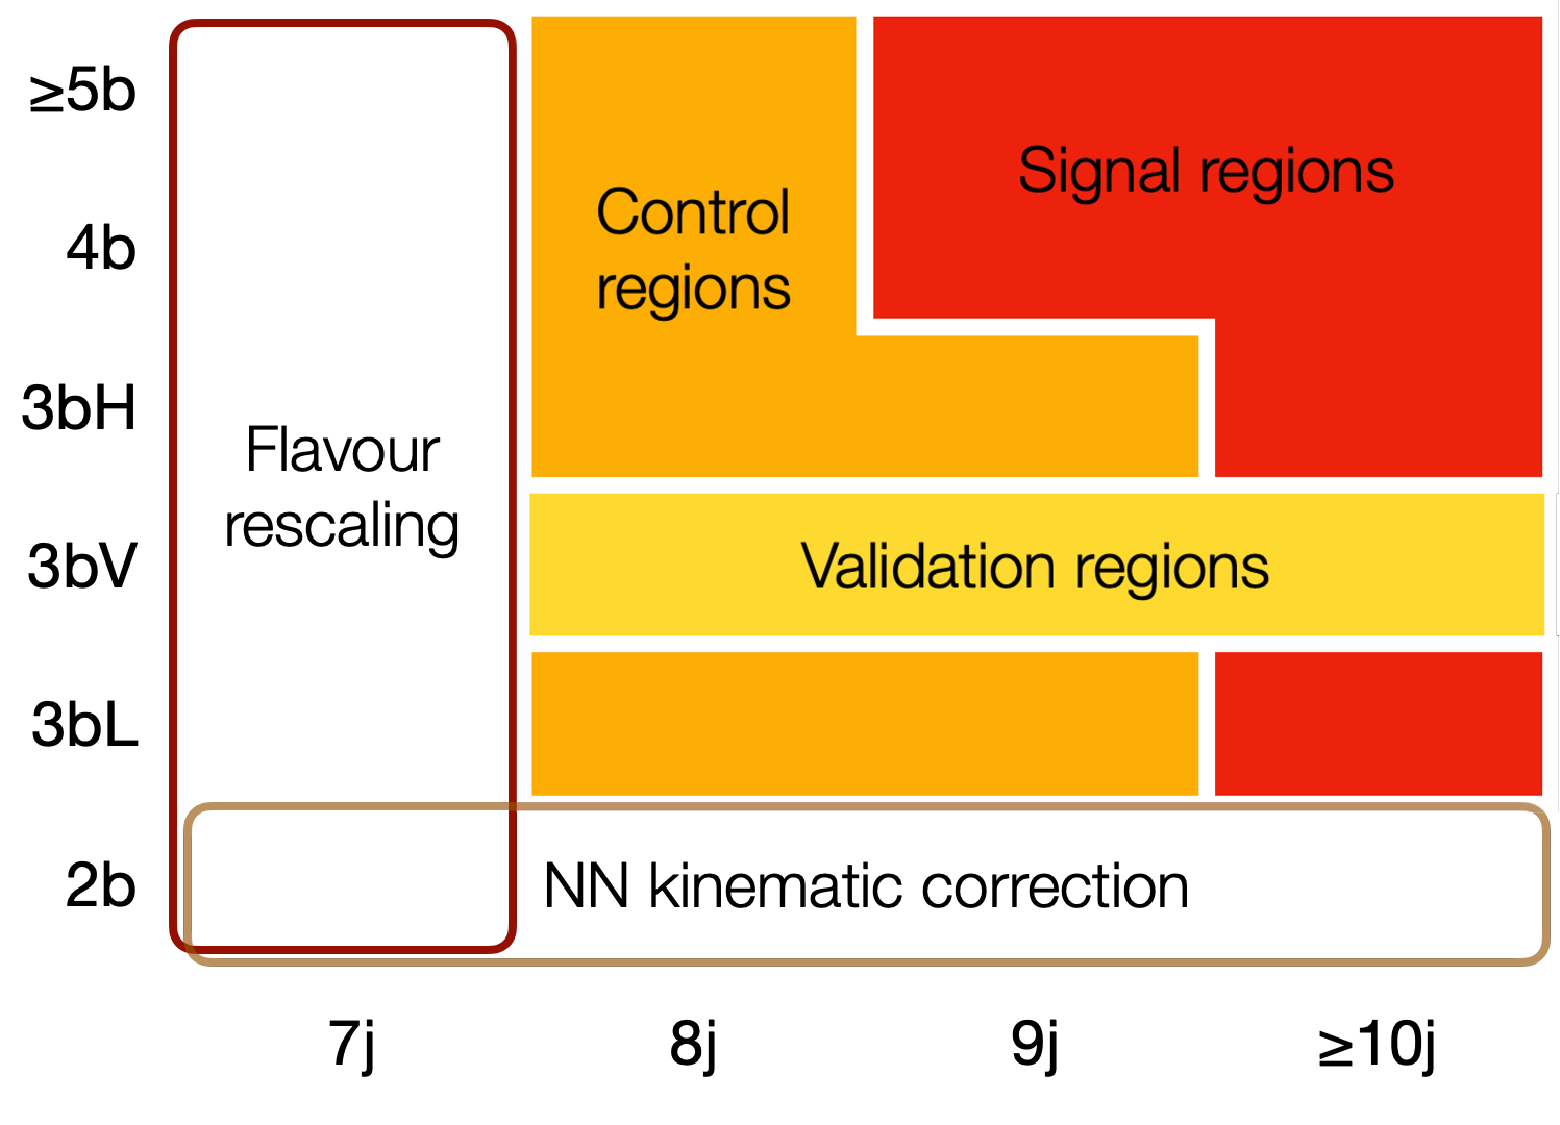
\includegraphics[width=0.48\textwidth]{figures/1l_regions.pdf}
  \hfill
  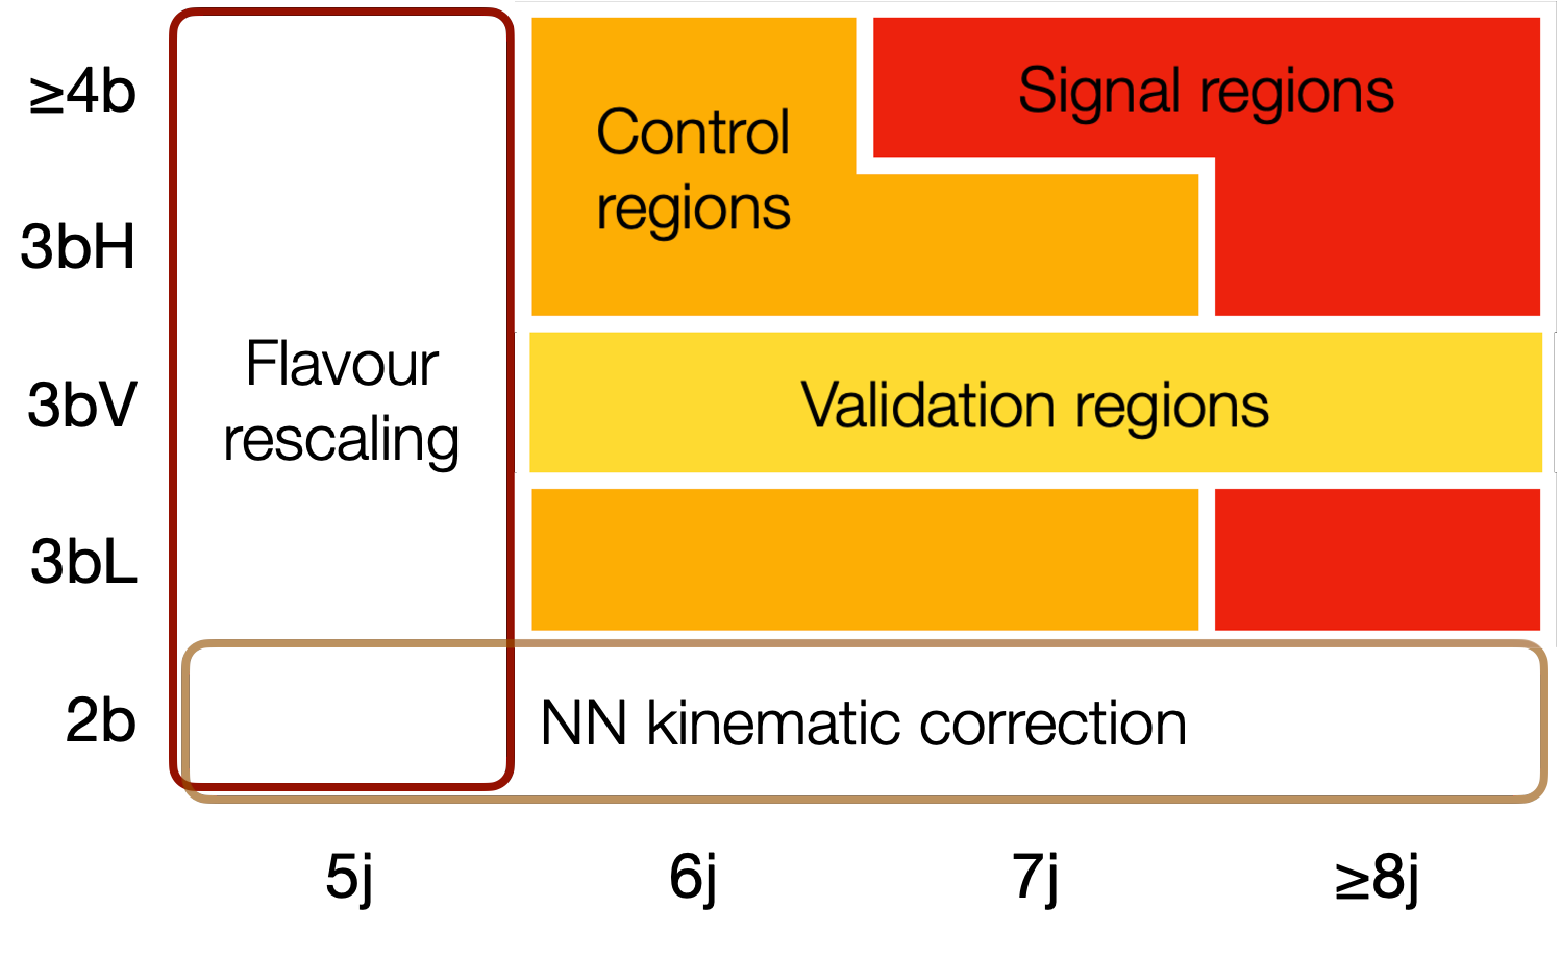
\includegraphics[width=0.48\textwidth]{figures/2los_regions.pdf}
  \caption{
    Schematic representation of the event categorisation
    in the 1L (left) and 2LOS (right) channels.
    The axes correspond to jet multiplicity and
    $b$-jet multiplicity requirements.
  }
  \label{fig:regions}
\end{figure}
%---------------------------------------------------------